%----------------------------------------------------------------------------
\chapter{Validáció}
\label{chp:validation}
%----------------------------------------------------------------------------
\begin{itemize}
  \item a két alfejezet rövid tartalma jön ide
\end{itemize}

%----------------------------------------------------------------------------
\section{Tesztelés}
%----------------------------------------------------------------------------
\begin{itemize}
  \item a készített alkalmazás egy adott bemenettel történő futását kísérjük nyomon:
  \item tesztkörnyezet bemutatása, milyen szempontok alapján lett összeállítva
  \item program futásának végigkövetése (sok screenshottal)
  \item értékelés
\end{itemize}

%----------------------------------------------------------------------------
\section{Teljesítményelemzés}
%----------------------------------------------------------------------------
A programom teljesítményének elemzéséhez a következő méréseket végeztem el:

\begin{itemize}
  \item 1,2,4 és 8 GiB méretű fájlok terítése 10 ill. 25 gépre
  \item 4 GiB méretű fájl terítése 25 gépre háromször, különbőző seed választásával
  \item Hibatűrési tesztek a terítés elején hiányző, ill. aközben kieső gépekkel.
\end{itemize}

Továbbá, hogy legyen összehasonlítási alap  az eredeti Chaincast alapú terítést is lefuttattam 25 gépre 1,2,4 és 8 GiB méretű fájlokkal.
A mérési eredmények az alkalmazásom futásakor keletkező logfájlból származnak, Chaincast esetében pedig a Jenkins webes felületén a terítéshez tartozó build ``build output'' részből.

\subsection{Chaincast és Torrent alapú terítés idejének összehasonlítása}

Nem a gyorsabb fájlterítés megvalósítása volt a programom egyik célja, de attól még érdemes lehet összehasonlítanunk a két módszer sebességét, hiszen mindegy mennyit nyerünk a robusztusságon , ha használhatatlanul lassabb lesz az alkalmazás a mostaninál. Az ~\ref{fig:chaincasttorrrentcomparison}-es~ábrán láthatjuk a különbőző méretű fájlok terítésének az idejét. Előtte visztont érdemes részletesebben megnézni, hogy ez az idő konkrétan mit (nem) tartalmaz:

\begin{itemize}
  \item Egyik megoldásnál sem tartalmazza a terítés ideje a terítendő fájlok létrehozását, és a központi gépre másolását (ami egyik esetben egy hálózati meghajtó, másik esetben a torrent-es terítés seed-je)
  \item Torrent-es terítésnél az időt a fájl hash-elése előtt, illetve után kezdjük mérni, Chaincast-nál a webes felületen a terítés indításától
\end{itemize}

Az előbbi állítások a későbbi mérésekre is igazak lesznek.

\begin{figure}[ht]
	\centering
	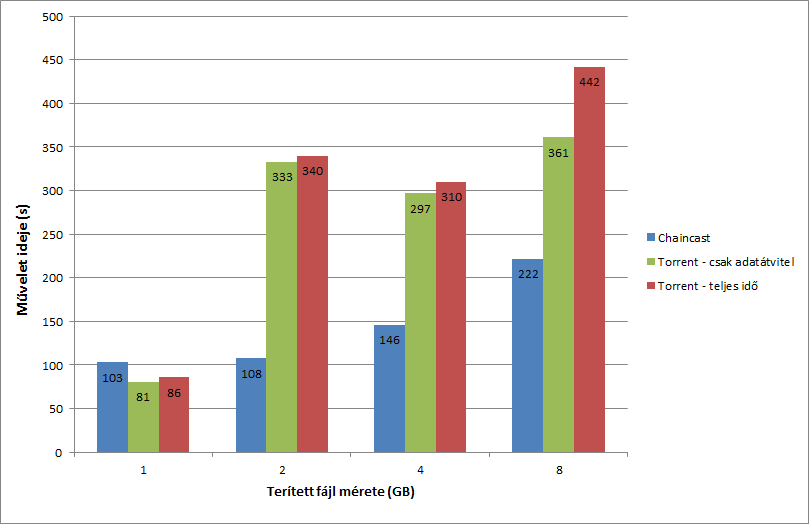
\includegraphics[width=150mm, keepaspectratio]{figures/Perf_chaincast_torrent_comparison.png}
	\caption{Chaincast és Torrent alapú terítés idejének összehasonlítása}
	\label{fig:chaincasttorrrentcomparison}
\end{figure}


Ide írom, hogy milyen következtetést kellene levonni az ábráról.
meglepó, hogy 2 g milyen lasssú, kis fájlnál nem nagyon van kül
nagyobb fájloknál kb 2x lassabb terítés , ez elfogadható, főleg hogy azt tapasztalam, hogy átlagosan 2 prbóálkozás kell egy sikeres chaincasthoz, ami ha a végém szakadna meg akkor hasonló időt vesz igénybe
esetleg még a hashelés által okozott overhead a fájl méretével egyenesen arányosan nő



\subsection{Következő alfejezet}

maradék téma:
\begin{itemize}
  \item letöltési sebességek torrent esetén, átlag és max
  \item különbőző seedek választása esetén a terítés sebességének összehasonlítása
  \item 10 vs 25 gépes torrentes terítés nagy összehasonlító táblázat
  \item torrentes terítések: leghamarabb és legkésőbb végzett gépek - annak megnézése, hogy előfordul-e hogy egy gép többször első, vagy utolsó lesz, ebből akár lehet következtetni hálózattal/gépekkel kapcsolatos szűk keresztmetszetekre
  \item hibatűrési mérések: elején hiányzó géppel, ill. terítés közben kiesőkkel
\end{itemize}

